
%\documentclass[conference,letterpaper,10pt]{IEEEtran}
\documentclass[journal,draftcls,onecolumn,12pt,twoside]{IEEEtran}
\newcommand{\folder}{/home/bohulu/Documents/texmf}
\input{\folder/hfiles/epaper}
\usepackage {graphics}
\usepackage{caption}
\usepackage{tabularx}

\begin{document}
\title{
A Method to Obtain Complete Information about Low-Weight Codewords of Recursive Systematic Convolutional Codes}
\author{%
  \IEEEauthorblockN{Bohulu~Kwame~Ackah~and~Chenggao~Han\\}
  \IEEEauthorblockA{Graduate School of Informatics and Engineering,\\
   The University of Electro-Communications,\\
    1-5-1 Chofugaoka, Chofu-shi, Tokyo, 182--8585, Japan\\
                    Email: \{bohulu, han.ic\}@uec.ac.jp}
}


\maketitle
%\begin{abstract}
%For the {\it turbo code} (TC) consisting of  {\it recursive systematic convolutional} (RSC) codes, the complete knowledge of the low-weight codewords of the component code is very important for interleaver design to achieve a good performance. In this paper, we present a method to obtain complete information about low-weight codewords for  RSC codes. For a given RSC code, we first identify the codewords with weight-$2$ and weight-$3$ {\it parity-check components} (PCs) based on the characteristic of the feed-forward polynomial and similarly, we identify the codewords with low-weight {\it systematic components} (SCs) based on the feedback polynomial. The low-weight codewords are established from the identified codewords. To validate our proposed method, we obtain a union bound using the established low-weight codewords and compare it with that obtained via the transfer function and the {\it bit error rate} (BER) curve drawn from simulation results.

%\end{abstract}
\begin{abstract}
	The  {\it recursive systematic convolutional} (RSC) code is widely used as the component code of high-performance error correcting codes and the complete knowledge of the low-weight codewords of the employed RSC code is very important for the construction of the code to achieve a good performance. In this paper, referring to the generator function of RSC code, we present a method to obtain complete information about low-weight codewords of RSC codes. To this end, we first identify the codewords with weight-$2$ and weight-$3$ {\it parity-check components} (PCs) based on the characteristic of the feed-forward polynomial, and similarly, those with low-weight {\it systematic components} (SCs) based on the feedback polynomial. The low-weight codewords are established from the identified codewords. To validate the proposed method, we obtain a union bound using the established low-weight codewords and compare it with that obtained via the transfer function and the {\it bit error rate} (BER) curve drawn from simulation results.
\end{abstract}
\section{Introduction}

The RSC code, developed by Punya Thitimajshima, was first introduced in the Claude Berrou's 1993 paper \cite{Berrou93-05C} as the 
{\it component code} (CC) for the then newly invented TC, which is one of the \textit{forward-error correcting} (FEC) codes that comes very close to satisfying the Shannon limit for AWGN channels.  2 years after \cite{Berrou93-05C}, \cite{Thitimajshima95-11C} was published, giving more details on the RSC code. Subsequently, \cite{Benedetto96-05J}, which detailed the inner workings of parallel concatenated codes, proved why RSC codes are better suited for use in the TC (better performance at any SNR for high code rate compared to other classes of convolutional codes) and in so doing, established them as the CC of choice for the TC.

Due to the success of the TC,  it has been adopted by many industral standards \cite{802-16e-04S}, \cite{dvb-rcs2-S},\cite{LTE-S} and the RSC code has been adopted as the CC for many other concatenated coding schemes. Examples include {\it recursive convolutional space-time codes} (ReC-STC) designed by adopting several parallel two-state RSC codes \cite{Ying05-07L}, a concatenated code obtained by combining a RSC code with a {\it Low-Density Parity-Check} (LDPC) code \cite{Gounai06-06C}, {\it binary self-concatenated convolutional codes employing iterative decoding} (SECCC-ID) with RSC codes as the CC \cite{Butt08-11C} and the {\it Reed-Solomon Convolutional Code} (RS-CC) concatenated code \cite{Xu07-04C}, \cite{Byun10-09C},\cite{Joshi11-11C}.  Despite the performance of these concatenated codes, the RSC code remains associated with the TC.

%RSC codes are used in concatenated codes as the binary inner code, where the codewords become the symbols to the outer non-binary code \cite{Proakis08B}. An example of such a code is the {\it Reed-Solomon Convolutional Code} (RS-CC) concatenated code, which is widely used various sysytems and widely researched \cite{Xu07-04C}, \cite{Byun10-09C},\cite{Joshi11-11C}, \cite{Joshi12-08C}. However, RSC codes were originally developed for use in parallel concatenation codes, and their most popular application is as the component code for TCs.

 The TC is generally constructed by concatenating two RSC codes (usually of the same kind) parallely  via an interleaver . A well designed TC realizes a large minimum distance via the interleaver, if it maps each bit sequence wit a  low-weight PC in the first RSC code onto that with a high-weight PC in the second RSC code.
Thus, the design of a good deterministic interleaver requires the complete knowledge of all the low-weight codeword component patterns of the employed RSC code and missing even one of these patterns may result in TC with subpar error correction performance.

The transfer function of an RSC code is an interleaver design tool that provides information about the different weights in the code, as well as their corresponding multiplicities (distance spectrum). 
However, it provides no information with regards to the pattern of the low-weight codeword components. As an added downside, the complexity of calculating the transfer function for a given RSC code increases with the number of states, and other methods such as Mason's Rule \cite{Moon05B} have to be used. Research into other methods for finding the distance spectrum have been carried out in recent years.  In \cite{Lu16-10C}, an algorithm for evaluating the input-parity weight distribution of
terminated RSC codes is presented, while in \cite{Deng17-01C}, the distance spectrum of tail-biting duo-binary
RSC codes is calculated using the modified FAST algorithm. These methods also do not reveal the pattern of the low-weight codeword components and to the best of our knowledge, there exists no interleaver design tool that provides complete knowledge of the low-weight codewords. Because of this, many of the interleaver design methods end up completely ignoring certain important low-weight codewords. In \cite{Sun05-01J} for example, the interleaver design method does not take into account the existence of low-weight codewords with systematic components of weight 3, especially for the $5/7$  RSC code, where such codewords are dominant.

In this paper, we propose a method to obtain complete information about the low-weight codeword components. The complexity of our proposed method is independent of the number of states of the RSC code and its ability to also reveal the low-weight codeword patterns of an RSC code makes it an excellent interleaver design tool.
We establish the low-weight codewords for the given RSC code by identifying codewords with either PCs or SCs of weight-2 and weight-3. Then, using the established low-weight codewords, we validate our proposed method by obtaining a union bound and comparing it to that obtained via the transfer function method and the BER curve obtained via simulation results.

The remainder of the research paper is organised as follows. Definitions used in this paper are introduced in Section \ref{secPrelim}. In Section \ref{sec2}, we discuss the characteristics of the low-weight RSC codewords and then present our method in Section \ref{sec3}. Validation of our proposed method for specific RSC codes as well as discussion of numerical results is done in Section \ref{sec4} and the paper concludes in Section \ref{sec6}.

\subsection{Notations}

For two positive integers $\alpha$ and $\beta$, the least common multiple of $\alpha$ and $\beta$ is dentoed as $\lcm(\alpha,\beta)$ while the remainder $\alpha$ divided by $\beta$ is denoted as $\alpha \mod \beta$. $\alpha | \beta$ implies $\alpha$ is a divisor of $\beta$. For an integer pair $(\alpha,~\beta)$, $(\alpha,~\beta) \bmod \epsilon_0$ is shorthand for the operation $(\alpha \bmod \epsilon_0,~\beta \bmod \epsilon_0)$. The sets of non-negative and positive integers are denoted by $\bbZ$ and $\bbZ^+$, respectively. For two integer sets $\bbM$ and $\bbN$, the tensor product that yields the set consisting of all pairs of $\bbM$ and $\bbN$ is denoted as $\bbM \otimes \bbN$ and we assume the elements in each resultant pair are sorted in increasing order. 



\section{Preliminaries}
\label{secPrelim}

A polynomial in $x$ with degree $M$ is an expression of the form
%and coefficients in $\cV$ is denoted by $v(x)$, and defined as 
\begin{equation}
v(x) = \sum_{m=0}^{M} v_mx^m
\label{Eq:polynomial}
\end{equation}
where $v_M \neq 0$ and $v_m,~0 \leq m \leq M$, are called the \textit{coefficients}. If $v_M=1,~v(x)$ is called a \textit{monic} polynomial. We say the total number of the non-zero coefficients of $v(x)$ is the \textit{Hamming weight} of $v(x)$, denoted as $w_H(v(x))$.

For a prime number $p$, if the addition and multiplication of two elements in the integer set $\{ 0,1,p-1\}$ are performed on the terms $\bmod~p$, we call the set a Galois field, denoted as $\GF(p)$. If the coefficients in \eqref{Eq:polynomial} are elements of $\GF(p)$, $v(x)$ is called a {\it polynomial over} $\GF(p)$.


For two polynomials $v(x)$ and $w(x)$ with degrees $M$ and $N$, respectively, the addition and multiplication over $\GF(p)$ are defined as 
\begin{align}
v(x)+w(x)=\sum_{m=0}^{\max\{ M,N\}} [(v_m +w_n)\mod p] x^m
\label{Eq:addition}
\end{align}
and
\begin{align}
v(x)w(x)=\sum_{m=0}^{ M+N} \sum_{i=0}^{m} [v_i w_{m-i}\mod p]x^m
\label{Eq:multiplication}
\end{align}
respectively. 

We say a monic polynomial is a \textit{prime polynomial} if it cannot be represented by multiplication of some lower degree polynomials.
For two polynomials $v(x)$ and $w(x)$ over $\GF(p)$, $w(x) \neq 0$, there exists polynomials $q(x)$ and $r(x)$ 
over $\GF(p)$ such that 
\begin{align}
v(x) = w(x)q(x)+r(x)
\label{Eq:decomposition}
\end{align}
with $\deg(r(x)) < \deg(w(x))$. We represent $r(x)$ in the expression \eqref{Eq:decomposition} as
\begin{align}
r(x) \equiv v(x)\mod w(x)
\end{align}
and call it the \textit{remainder polynomial}, while $q(x)$ is called the \textit{quotient polynomial} of the division of $v(x)$ by $w(x)$.

Let $v(x)$ be a prime polynomial over $\GF(p)$ with $\deg(v(x)):=M>1$ and $\cV$ be the polynomial set of size $p^M$ containing all polynomials over $\GF(p)$ with degree less than $M$. Then, the \textit{extension field of $\GF(p)$}, denoted by $\GF\left(p^M\right)$, is the set $\cV$ with addition and multiplication over $\GF(p)$, where the multiplication is carried out modulo-$v(x)$ over $\GF(p)$.
Each non-zero element in $\GF \left(p^M\right)$ can be represented by a power of $x$ uniquely as $x^m,~0 \leq m \leq p^M-1$. %, where $X^2$ may be used in place of $1+x$, for example.
%Through out this paper, the polynomilal nad power notations will be used more often for the sake of convenience, with the appropriate conversion between the power and polynomial notation made known where necessary.  

For each non-zero element of $\GF \left(p^M\right)$, there exist integers $\epsilon$ such that $x^{\epsilon}=1$ and the least positive integer among them is called the \textit{order} of $x$. We say that elements with order $\epsilon=p^M-1$ are \textit{primitive elements}. For $\GF \left(p^M\right)$ generated by a prime polynomial $v(x)$ with $\deg(v(x))=M$, if $x$ is a primitive element in $\GF \left(p^M\right)$, then  $v(x)$ is called a \textit{primitive polynomial}. 
%
Finally, the root of $v(x)$, is the non-zero element $\varphi,~\varphi \in \GF \left(p^M\right)$ such that $v(\varphi)=0$. If $v(x)$ is a primitive polynomial, the order of $\varphi$ is $\epsilon=p^M-1$, otherwise $\epsilon | p^M-1$. 
Moreover, the elements $\varphi^i,~0 \leq i \leq \epsilon -1$, are all distinct from each other.
 
%Finally, let $(e,~f)$ represent a pair of non-zero positive integers. Then $(e,~f) \bmod 2^M-1$ is shorthand for the operation $(e \bmod 2^M-1,~f \bmod 2^M-1)$.


\section{The characteristics of the low-weights codewords of RSC code}
\label{sec2}
The outputs of an RSC code are determined by the input bit sequence $b(x)$, states of the shift registers and feedforward and feedback connections of the shift registers that can be represented by a generator function. 

As an instance,  the generator function of a rate $1/2$ RSC code may be written as  $$\left[1 ~\frac{f(x)}{g(x)}\right]$$ where $1$ yields the \textit{systematic  component} (SC) $b(x)$ while the \textit{parity-check component} (PC) $h(x)$ is associated with the feedforward and feedback connections of the shift registers, specified by $f(x)$ and $g(x)$, respectively. The output $c(x)$ is the mixture of the SC and PC as
\begin{equation}
c(x) = b(x^2)+xh(x^2)
\label{codeword-comp}
\end{equation}
where 
\begin{equation}
h(x) =f(x)g^{-1}(x)b(x)
\label{eq:parity-def}
\end{equation}
From \eqref{codeword-comp}, it is trivial that
\begin{equation}
w_H(c(x))=w_H(b(x)) + w_H(h(x))
\label{eq:cw-weight}
\end{equation}
and hence, each low-weight codeword is combination of low-weight SC and PC.

Under the assumption of large frame sizes, the presence of $g^{-1}(x)$  in \eqref{eq:parity-def} may involve a particular bit sequence that repeats a large number of times, hence yielding a high-weight PC. Therefore low-weight PCs occur if and only if
\begin{equation}
b(x) \bmod g(x) \equiv 0
\label{eq:rtz-input}
\end{equation}
The bit sequences satisfying \eqref{eq:rtz-input} are called \textit{return-to-zero} (RTZ) input. Thus, every RTZ input can be factorized as  
\begin{equation}
b(x) =a(x)g(x)
\label{eq:low-weight-msg}
\end{equation}
and, substituting (\ref{eq:low-weight-msg}) into \eqref{eq:parity-def}, we can characterize the low-weight PC as
\begin{equation}
\begin{split}
h(x)&=f(x)\cdot g^{-1}(x)\cdot a(x)g(x)\\
&=a(x)f(x)
\end{split}
\label{eq:low-weight-parity}
\end{equation}
Therefore, in this paper, we attempt to find $a(x)$s satisfying  \eqref{eq:low-weight-msg} and  \eqref{eq:low-weight-parity} simultaneously for low-weight $b(x)$ and $h(x)$, respectively. 
%
However, since there is no essential mathematical difference between the two equations, in the next section, we present a method for determining the low-weight PC patterns for $w_H(h(x))= 2,3$.
\section{The patterns of the low-weight PCs}
\label{sec3}
We assume $f(x)$ can be factorized into $K$ prime polynomials as 
\begin{align}
f(x)&=\prod_{k=0}^{K-1}f_k^{\gamma_k}(x)
\label{Eq:GeneralForm}
\end{align}
where $\gamma_0,\gamma_1,\cdots,\gamma_{K-1}$ are positive integers and let $\varphi_k$ be a root of $f_{k}(x)$ of order $\epsilon_k$. After that, we consider the solution of
\begin{align}
	h(x) \mod f(x) \equiv 0
	\label{Eq:condition}
\end{align}

We start from the simplest case $K=1$, \ie, $f(x) = f_0^{\gamma_0}(x)$. Then, \eqref{eq:low-weight-parity} indicates that each root of $f(x)$ is also the root of $h(x)$ and we distinguish the cases $\gamma_0 = 1$ and $\gamma_0 > 1$. For the former case, since all $\varphi_0^i$, $0 \leq i < \epsilon_0$, are distinct from each other, the equation
\begin{align}
	h(\varphi_0^i)=0,~~~ 0 \leq i < \epsilon_0
	\label{Eq:rootcondition}
\end{align}
is a necessary and sufficient condition of \eqref{Eq:condition} while it is necessary but not sufficient for the latter case. Thus, for the case $\gamma_0 >1$, we obtain extra conditions using differential equations as
\begin{align}
\left.\frac{d^{(j)}h(x)}{d x^j}\right|_{x=\varphi_0^i}=0,~~~0 \leq i < \epsilon_0,~1 \leq j < \gamma_0
\label{Eq:differential}
\end{align}
where the derivation is calculated using the {\it Hasse derivative} defined as
\begin{align}
\frac{d^{j}x^k}{dx^j}=
	\begin{cases}
	\left({}_kC_j\mod 2\right)x^{k-j}, & k \geq j\cr
	0, & \mathotherwise
	\end{cases}
\end{align}
for the bionomial coefficient ${}_kC_j$.

For the case where $K>1$, we may repeat the above discussion for the roots $\varphi_k$, $0 < k < K$, and take the intersection of the results to determine the low-weight PCs.

\subsection{The weight-2 PCs}
\label{sec:PC2}
Each weight-2 PC can be written as 
\begin{equation}
h(x)=1+x^{\alpha}
\label{eq:wt2-gen-form}
\end{equation}
without loss of generality. Thus, we have from \eqref{Eq:rootcondition} that
\begin{equation}
(\varphi_0^i)^{\alpha} =1,~~~ 0 \leq i < \epsilon_0
\label{novelEq5b}
\end{equation}
On the other hand, the order of $\varphi_0$ is the least integer satisfying $\varphi_0^{\epsilon_0} = 1$. Thus, $\alpha$ should satisfy the condition
\begin{equation}
\alpha \equiv 0 \mod \epsilon_0~~~\mathor~~~\epsilon_0|\alpha
\label{eq:wt2-alpha}
\end{equation}

\subsection{The weight-3 PCs}

Without loss of generality, the weight-3 PCs can be written as 
\begin{equation}
h(x)=1+x^{\alpha}+x^{\beta},~\alpha < \beta
\label{novelEqwt3}
\end{equation}
and hence, $(\alpha,\beta)$ should satisfy the condition
\begin{equation}
\varphi_0^{\alpha}+\varphi_0^{\beta}= 1
\label{Eq:novelEq5b}
\end{equation}
The pairs $(\alpha, \beta)$ satisfying \eqref{Eq:novelEq5b} can be found by referring to the table of the extended field for $\GF\left(2^M\right)$. 
Let $(m,n)$ be such a pair and let $\bbM=\{\epsilon_0 \ell+m\}_{\ell \in \bbZ}$ and $\bbN=\{\epsilon_0 \ell+n\}_{\ell \in \bbZ}$. Then it is obvious that each pair $(\alpha,~\beta) \in \bbM \otimes \bbN$ satisfies
\eqref{Eq:novelEq5b}. For a fixed $\alpha$, on the other hand, since $\alpha+i$, $0 \leq i < \epsilon_0$, are distinct from each other, any integer $\beta$ that satisfies \eqref{Eq:novelEq5b} must be such that $n\equiv \beta \mod \epsilon_0$.

%Furthermore, let  We denote the set of all pairs as $\bbM \bar{\otimes} \bbN$, where the elements of this set are formed using a tensor product approach. Then, $(\alpha,~\beta) \in \bbM \bar{\otimes} \bbN$
\subsection{Examples}

In the following, we present some examples of the proposed method to determine weight-2 and weight-3 PCs for several feedfoward polynomials of form given in \eqref{Eq:GeneralForm}. For the case $K=1$, Examples \ref{Ex:1} and \ref{Ex:2} are two instances where $f(x)$ is a primitive polynomial while an instance where $f(x)$ is prime but not a primitive polynomial is given in Example \ref{Ex:3}. Example \ref{Ex:4} demonstrate the case $\gamma_0 > 1$, and Examples \ref{Ex:5} and \ref{Ex:6} are two instances of the case $K=2$. Some weight-$2$ and weight-$3 ~ h(x)$ are compiled in Table \ref{examples-table} with their corresponding $a(x)$ for reference.

\subsubsection{$f(x)$ is a primitive polynomial}

\begin{example}$f(x)=1+x+x^2$
	
Since $x^1=x$, $x^2 \equiv 1+x \mod f(x)$, and $x^3 \equiv 1 \bmod f(x)$, $f(x)$ is a primitive polynomial with a root of order $\epsilon_0=3$. Thus, $\alpha$ in the weight-2 PCs shown in \eqref{eq:wt2-gen-form} should be a multiple of $3$ as $h(x)=1+x^{3\ell}$, $\ell \in \bbZ^+$, while the corresponding $a(x)$ can be expressed by 
\begin{equation*}
	a(x)=\sum_{i=0}^{\ell-1} x^{3i}(1+x)
\end{equation*}

To determine the weight-3 PCs, we can see from Table \ref{novelTab7} that there is a pair $(1,2)$ satisfying $x^1+x^2 \equiv 1 \mod f(x)$. Thus, let $\bbM = \{3\ell+1\}_{\ell \in \bbZ}$ and $\bbN = \{3\ell+2\}_{\ell \in \bbZ}$. Then, we have $x^\alpha+x^\beta \equiv 1 \mod f(x)$ for each $(\alpha,\beta) \in \bbM\otimes\bbN$.
\label{Ex:1}
\end{example}

\begin{table}[htbp]
	\caption{Non-zero Elements of $\GF \left(2^2\right)$ generated by $f(x)=1+x+x^2$}
	\centering
	\begin{tabular}{c c} 
		\toprule
		power representation & polynomial representation \\ [0.5ex] 
		\midrule
		$x^0~=x^3=1$ & $1$\\
		\hline
		$x$ & $x$\\
		\hline
		$x^2$ &  $1+x$\\
		\bottomrule
	\end{tabular}
	\label{novelTab7}
\end{table}

\begin{example}	$f(x)= 1+x+x^4~$
	
	Since $f(x)$ is a primitive polynomial with a root of order $\epsilon_0=2^M-1=15$, the weight-2 PCs have the form
	$h(x)=1+x^{15\ell}$
	while the corresponding $a(x)$ can be expressed as 
	$$ a(x) = \sum_{i=0}^{\ell} x^{15i} \left(1 +x +x^2 +x^3+x^5+x^7+x^8+x^{11} \right)$$
	
	For the weight-3 PCs, we refer to Table \ref{GF-tables} and observe that there are 7 $(m,n)$ pairs which satisfy $x^m+x^n \equiv 1 \mod 15$. Thus, $(\alpha,~\beta) \in \bigcup_{i=0}^6 \bbM_i\otimes\bbN_i$ satisfies \eqref{novelEqwt3}, where
	\begin{align}
	\bbM_0 &:= \{15\ell + 1\}_{\ell \in \bbZ},~\bbN_0 := \{15\ell + 4\}_{\ell \in \bbZ}\cr
	\bbM_1 &:= \{15\ell + 2\}_{\ell \in \bbZ},~\bbN_1 := \{15\ell + 8\}_{\ell \in \bbZ}\cr
	\bbM_2 &:= \{15\ell + 3\}_{\ell \in \bbZ},~\bbN_2 := \{15\ell + 14\}_{\ell \in \bbZ}\cr
	\bbM_3 &:= \{15\ell + 5\}_{\ell \in \bbZ},~\bbN_3 := \{15\ell + 10\}_{\ell \in \bbZ}\cr
	\bbM_4 &:= \{15\ell + 6\}_{\ell \in \bbZ},~\bbN_4 := \{15\ell + 13\}_{\ell \in \bbZ}\cr
	\bbM_5 &:= \{15\ell + 7\}_{\ell \in \bbZ},~\bbN_5 := \{15\ell + 9\}_{\ell \in \bbZ}\cr
	\bbM_6 &:= \{15\ell + 11\}_{\ell \in \bbZ},~\bbN_6 := \{15\ell + 12\}_{\ell \in \bbZ}
	\end{align}
	\label{Ex:2}	
\end{example}

\subsubsection{$f(x)$ is a prime but not primitive polynomial}

\begin{example}
$f(x)=1+x+x^2+x^3+x^4$

Since $x\equiv x^5 \mod f(x)$ as shown in Table \ref{GF-tables}, $\epsilon_0=5< 15$ and the weight-2 PCs can be expressed as $h(x)=1+x^{5\ell}$, $\ell \in \bbZ^+$. For weight-3 PCs, on the other hand, Table \ref{GF-tables} indicates that there is no pair $(m,~n)$ satisfying $x^m+x^n \equiv 1$, and hence, the given $f(x)$ does not yield any weight-3 PCs.
\label{Ex:3}
\end{example}

\subsubsection{$K=1$ and $\gamma_0 > 1$}
\begin{example}
	$f(x)=1+x^2$ and $f(x)=1+x^4$\newline
	
	If we rewrite the polynomials as $f(x)=(1+x)^2$ and $f(x)=(1+x)^4$,	the order of the root $\varphi_0$ is $\epsilon_0=1$. 
	Thus, each $\alpha \in \bbZ^+$ should satisfy
	\begin{align}
		h(x) = 1+x^\alpha = 0
	\end{align}
	However, the following second order differential equation
	\begin{align}
	\frac{dh(x)}{dx} = (\alpha\mod 2) x^{\alpha-1} = 0
	\end{align}
	implies $\alpha$ should be an even number. Therefore, for the case $f(x) = 1+x^2$, we write the PCs as  $h(x)=1+x^{2\ell}$, $\ell \in \bbZ^+$.
	

	For the case $f(x) = 1+x^4$, from \eqref{Eq:differential}, we have
	\begin{align}
		\begin{cases}
		\frac{d^2h(x)}{dx^2} = \left[\frac{\alpha(\alpha-1)}{2} \mod 2\right]x^{\alpha-2} = 0 \\
		\frac{d^3h(x)}{dx^3} = \left[\frac{\alpha(\alpha-1)(\alpha-2)}{6} \mod 2\right]x^{\alpha-3} = 0
		\end{cases}
		\label{Eq:Ex3Diff}
	\end{align}
	and $\alpha=4\ell$, $\ell \in \bbZ^+$, satisfies \eqref{Eq:Ex3Diff} simultaneously.
	
	Since $\GF(2)$ has single non-zero element, it does not provide a pair $(m,~n)$ satisfying $x^m+x^n = 1$ and, consequently, there are no weight-3 PCs associated with $f(x)$.
\label{Ex:4}
\end{example}

\subsubsection{The case $K=2$}

For this case, we write the feedforward polynomial as $f(x) =f_0(x)f_1(x)$ and give two examples.
\begin{example}
	$f(x)= (1+x)(1+x+x^3)=1+x^2+x^3+x^4$\newline
	
	Let $f_0(x)=1+x$ and $f_1(x)=1+x+x^3$. We know that the PCs  associated with $f(x)$ are intersection of those with $f_0(x)$ and with $f_1(x)$. 
	Since $f_0(x)$ does not yields any weight-3 PCs as explained in the Example \ref{Ex:4}, there are no such PCs associated with $f(x)$.
	
	With respect to the weight-2 PCs, from Example \ref{Ex:4}, $\epsilon_0=1$ and $\epsilon_1=7$. We have $\lcm(\epsilon_0,\epsilon_1)=7$ and
	$h(x) =1+x^{7\ell}$
	with the corresponding $a(x)$ given by
	$$a(x) = \sum_{i=0}^{\ell-1} x^{7i}(1+x^2+x^3)$$
	\label{Ex:5}	
\end{example}

\begin{example}
$f(x)=(1+x+x^2)(1+x^2+x^3)=1+x+x^5$

For this case, it is not difficult to see that $\epsilon_0=3$ and $\epsilon_1=7$ for $f_0(x)=1+x+x^2$ and $f_1(x)=1+x^2+x^3$, respectively. Thus, from $\lcm(\epsilon_0,\epsilon_1)=21$, the weight-2 PCs have the general form of $h(x)=1+x^{21\ell}$, $\ell \in \bbZ^+$, while the corresponding $a(x)$ can be expressed as $$a(x)=\sum_{i=0}^{\ell-1} x^{21i}(1+x^2+x^3+x^4+x^6+x^8+x^{4}+x^{6}+x^{8}+x^{11}+x^{12}+x^{16})$$.


In order to determine weight-3 PCs, we rewrite $\bbM$ and $\bbN$ in Example \ref{Ex:1} as $\bbM^0$ and $\bbN^0$, respectively,
and referring to Table \ref{GF-tables}, let
\begin{align}
	\bbM_0^1 &:= \{7\ell + 1\}_{\ell \in \bbZ},~\bbN_0^1 := \{7\ell + 5\}_{\ell \in \bbZ}\cr
	\bbM_1^1 &:= \{7\ell + 2\}_{\ell \in \bbZ},~\bbN_1^1 := \{7\ell + 3\}_{\ell \in \bbZ}\cr
	\bbM_2^1 &:= \{7\ell + 4\}_{\ell \in \bbZ},~\bbN_2^1 := \{7\ell + 6\}_{\ell \in \bbZ}
\end{align}

Then, we have
\[
(\alpha_0,~\beta_0) \in \bbM^0\otimes\bbN^0 
\]
and
\begin{equation*}
\begin{split}
(\alpha_1,~\beta_1) \in &\bigcup_{i=0}^2 \bbM_i^1\otimes\bbN_i^1 
\end{split}
\end{equation*}
Therefore, by taking the intersection, we can identify $(\alpha,\beta) \in \left(\bbM^0\otimes\bbN^0\right)\bigcap\left(\bigcup_{i=0}^2 \bbM_i^1\otimes\bbN_i^1 \right) $.
\label{Ex:6}
\end{example}

%=====Merged Example Tables =====
\begin{table}[htbp]
\caption{$a(x)$ and $h(x)$ for various $f(x)$}
\centering
\begin{tabularx}{0.48\textwidth}{l|cXl} 
\toprule
$f(x)$ & weight & $a(x)$ & $h(x)$\\
\midrule
 &  & $1+x$ & $1+x^{3}$ \\
&  &$1+x+x^3+x^4$ & $1+x^{6}$  \\
& 2 &$1+x+x^3+x^4+x^6+x^{7}$ &  $1+x^{9}$ \\
$1+x+x^2$&& $1+x+x^3+x^4+x^6+x^{7}+x^9+x^{10}$&  $1+x^{12}$ \\
\cline{2-4}
(Ex. \ref{Ex:1})& &$1$ & $1+x+x^2$\\ 
& 3&$1+x+x^2$ &  $1+x^2+x^4$\\
& &$1+x+x^3$ & $1+x^4+x^5$\\
& &$1+x^2+x^3$ & $1+x+x^5$ \\
\cline{1-4}
$1+x+x^4$&2& $1 +x +x^2 +x^3+x^5+x^7+x^8+x^{11}$&  $1+x^{15}$ \\
\cline{2-4}
(Ex. \ref{Ex:2})& &$1$ & $1+x+x^4$\\ 
& 3&$1+x+x^4$ &  $1+x^2+x^8$\\
& &$1+x+x^2+x^3+x^5$ & $1+x^7+x^9$\\
& &$1+x+x^2+x^3+x^6$ & $1+x^5+x^{10}$ \\
\cline{1-4}
&&$1+x$ &$1+x^5$\\ 
$1+x+x^2+x^3+x^4$&2&$1+x+x^5+x^6$ &$1+x^{10}$  \\
(Ex. \ref{Ex:3})&&$1+x+x^5+x^6+x^{10}+x^{11}$ & $1+x^{15}$ \\
&&$1+x+x^5+x^6+x^{10}+x^{11}+x^{15}+x^{16}$ &$1+x^{20}$  \\
\cline{1-4}
&&$1$ & $1+x^2$\\ 
$1+x^2$&2&$1+x^2$ & $1+x^4$ \\
(Ex. \ref{Ex:4})&&$1+x^2+x^4$ & $1+x^6$\\
&&$1+x^2+x^4+x^6$ & $1+x^8$\\
\cline{1-4}
&&$1$ & $1+x^4$\\ 
$1+x^4$&2&$1+x^4$ & $1+x^8$ \\
(Ex. \ref{Ex:4})&&$1+x^4+x^8$ & $1+x^{12}$\\
&&$1+x^4+x^8+x^12$ & $1+x^{16}$\\
\cline{1-4}
$1+x^2+x^3+x^4$&&$1+x+x^2$& $1+x^{7}$ \\
(Ex. \ref{Ex:5})&2&$1+x^2+x^3+x^7+x^9+x^{10}$	& $1+x^{14}$ \\
\cline{1-4}
&2&$1+x^2+x^3+x^4+x^6+x^8+x^{4}+x^{6}+x^{8}+x^{11}+x^{12}+x^{16}$ &  $1+x^{21}$\\
\cline{2-4}
$1+x+x^5$&&$1$ & $1+x+x^{5}$\\ 
(Ex. \ref{Ex:6})&3&$1+x+x^5$ &  $1+x^2+x^{10}$\\
&&$1+x+x^2+x^3+x^4+x^{6}+x^{8}$ & $1+x^{11}+x^{13}$\\
\bottomrule
\end{tabularx}
\label{examples-table}
\end{table}
%=====End Of Merged Example Tables =====






%===== Merged GF(2^M) tables=======
\begin{table}[htbp]
\caption{Galois Field Elements for various prime polynomials $f(x)$}
\centering
\begin{tabularx}{0.48\textwidth}{X|c|c|c} 
\toprule
\multicolumn{1}{c|}{Power Representation}&\multicolumn{3}{c}{polynomial representation}\\
\cmidrule(lr){1-4}
Generator polynomial &$1+x^2+x^3$&$1+x+x^2+x^3+x^4$&$1+x+x^4$\\
\cmidrule(lr){1-4}
$x^0$			&1				&1                                              &1\\
$x$			&$x$			&$x$                                                              &$x$\\
$x^{2}$		&$x^2$		&$x^2$                                                  	  &$x^2$\\
$x^{3}$		&$1+x^2$		&$x^3$                                                        &$x^3$\\
$x^{4}$ 		&$1+x+x^2$   &$1+x+x^2+x^3$ 					 	& $1+x$\\
$x^{5}$		&$1+x$		&                                                                   &$x+x^2$\\
$x^{6}$		&$x+x^2$		&                                                                   &$x^2+x^3$\\
$x^{7}$		&				&                								&$1+x+x^3$\\
$x^{8}$		&				&										&$1+x^2$\\
$x^{9}$		&				&										&$x+x^3$\\
$x^{10}$		&				&										&$1+x+x^2$\\
$x^{11}$		&				&										&$x+x^2+x^3$\\
$x^{12}$		&				&										&$1+x+x^2+x^3$\\
$x^{13}$		&				&										&$1+x+x^3$\\
$x^{14}$		&				&										&$1+x^3$\\
\bottomrule
\end{tabularx}

\label{GF-tables}
\end{table}

%=====End of Merged GF(2^M) tables=======
 








\section{validity confirmation through Union Bound}
\label{sec4}
 In this section, in order to confirm the validity of our proposed method, we obtain a union bound using the low-weight codewords with weight-$2$ and weight-$3$ PC or SC and compare it with that obtained via the transfer function as well as simulation results.

\subsection{A novel union bound}
Let $\bbA_h(d)$ be the set of all $a(x)$ which yields weight-$d$ PCs \ie, $w_H(h(x))=w_H(a(x)f(x))=d$. Similarly, we also define $\bbA_b(d)$ and $\bbA_c(d)$ as the sets of all $a(x)$s which result in weight-$d$ SCs and codewords, respectively.

Then, for $w_H(b(x)), w_H(h(x)) \geq 2$, we have from \eqref{eq:cw-weight} that
\begin{align}
\bbA_c(d) = \bigcup_{\ell = 2}^{d-2} \left\{\bbA_b(\ell) \cap \bbA_h(d-\ell)\right\}
\label{Eq:exactset}
\end{align}
Now, we replace the set $\bbA_c(d)$ by the following approximated set %\eqref{setApprox}
\begin{equation}
\begin{split}
\bbA_c(d) \approx \bbA_c'(d) &= \left\{\bigcup_{\ell = 2}^{\ell+1} \left\{\bbA_b(\ell) \cap \bbA_h(d-\ell)\right\}\right\} \\ 
&\bigcup \left\{\bigcup_{\ell = 2}^{\ell+1} \left\{\bbA_b(d-\ell) \cap \bbA_h(\ell)\right\}\right\}
\end{split}
\label{setApprox}
\end{equation}
and obtain an approximated union bound as
\begin{align}
P_b \leq \frac{1}{k} \sum_{d=d_{\text{free}}}^{d_{\text{free}+1}} \sum_{a(x) \in \cA'_c(d)}w_H(a(x)g(x)) Q\Bigg( \sqrt{\frac{2dE_c}{N_0}}\Bigg)
\label{novelEq7}
\end{align}
Notice that since $\bbA_c(d)$ in \eqref{Eq:exactset} is replaced by $\bbA_c'(d)$, the contributions of the codewords with $\ell \approx d-\ell$ may be neglected in our approximation.

To obtain $\bbA_c'(d)$, based on $f(x)$, we first generate the set consisting of $a(x)$s which yield the weight-2 and -3 PCs, \ie~$\bbA_h(2)\cup\bbA_h(3)$. Next, for each $a(x) \in \bbA_h(2)\cup\bbA_h(3)$, we determine the corresponding SC $b(x)=a(x)g(x)$. Similarly, we determine the PC $h(x)=a(x)f(x)$ for each $a(x)$ in the set $\bbA_b(2)\cup\bbA_b(3)$  obtained based on $g(x)$. Finally, we narrow down the corresponding codewords as $w_H(b(x))+w_H(h(x)) \leq d_{\text{free+1}}$ for $a(x) \in \bbA_h(2)\cup\bbA_h(3)\cup\bbA_b(2)\cup\bbA_b(3)$.

As examples, in Table \ref{code-tables-1},\ref{code-tables-2} and \ref{code-tables-3}, we listed the low-weight PCs and SCs found by our proposed method for the codes listed in Table \ref{TB:Codes} with the corresponding example numbers where each polynomial appeared in.
\begin{table}[htbp]
	\caption{The generator polynomials}
	\centering
	\begin{tabular}{cll} 
		\toprule
			& $f(x)$ & $g(x)$ \\ %[0.5ex] 
		\midrule
		Code I & $1+x^2$ & $1+x+x^2$\\
		(5/7) &  (Ex. \ref{Ex:4}) &  (Ex. \ref{Ex:1}) \\\hline
		Code I& $1+x+x^2+x^3+x^4$& $1+x^4$\\
		(37/21) &  (Ex. \ref{Ex:3}) &  (Ex. \ref{Ex:4})\\\hline
		Code III& $1+x+x^4$& $1+x^2+x^3+x^4$\\
		(23/35) &  (Ex. \ref{Ex:2}) &  (Ex. \ref{Ex:5})\\
		\bottomrule
	\end{tabular}
	\label{TB:Codes}
\end{table}

\subsection{Numerical results}

We obtained the approximated union bound by \eqref{novelEq7} for the codes listed in Table \ref{TB:Codes}. Since the codewords with the weights larger than $d_{\rm free+1}$ are neglected in our approximation, we also obtained the union bounds obtained using the codewords with weights up to $d_{\rm free+i}$, $0 \leq i \leq 3$, and compared them with that obtained using transfer function in Figures \ref{simFig1}-\ref{simFig3}.
For reference purpose, the details of the PCs and SCs used for drawing the bound are listed in Tables \ref{code-tables-1} - \ref{code-tables-3} with the extra codewords found by computer search (labelled as `Not Found').
In these figures, we also evaluated BER through computer simulations. To plot BER points, we assume each RSC code is BPSK modulated and transmitted over the AWGN channel with a frame with size of $N=64$. At the receiver, the Viterbi algorithm is used to recover the transmitted bits and we accumulated more than 1,000 bits errors for obtain each plot point.

\begin{table}[htbp]
		\caption{SCs and PCs for Code I}
		\centering
		\begin{tabularx}{0.48\textwidth}{|c|c|XXX} 
			\toprule
			$w_H(c(x))$&~& $a(x)$ & $b(x)$ & $h(x)$ \\ %[0.5ex] 
			\midrule
			5&Found&$1$ & $1+x+x^{2}$ & $1+x^2$\\
			\cline{1-5}
			6& ~&$1+x$ & $1+x^3$ & $1+x+x^2+x^3$\\
			&~ &$1+x^2$ & $1+x+x^3+x^4$ & $1+x^{4}$\\
			&Found&$1+x+x^2$ & $1+x^2+x^4$ & $1+x+x^3+x^4$\\
			&~&$1+x+x^3$ & $1+x^4+x^5$ & $1+x+x^2+x^5$\\
			\cline{1-5}
			7&Found&$1+x^2+x^3$ & $1+x+x^5$ & $1+x^3+x^4+x^5$\\
			&~&$1+x^2+x^4$ & $1+x+x^3+x^5+x^6$ & $1+x^{6}$\\			
			\cline{1-5}
			&~&$1+x+x^3+x^4$ & $1+x^6$ & $1+x+x^2+$\\
			&Found&&&$x^4+x^5+x^6$\\
			&~&$1+x^2+x^4+x^6$ & $1+x+x^3+x^5+x^7+x^8$ & $1+x^8$\\
			\cline{2-5}
			8&&$1+x+x^2+x^3$ 		&$1+x+x^3+x^5$ 		& $1+x+x^4+x^5$\\
			&&$1+x+x^2+x^4$ 		&$1+x^2+x^5+x^6$		& $1+x+x^3+x^6$\\
			&Not Found&$1+x+x^3+x^5$ 		&$1+x^4+x^6+x^7$ 		& $1+x+x^2+x^7$\\
			&&$1+x^2+x^3+x^4$ 	&$1+x+x^4+x^6$ 		& $1+x^3+x^5+x^6$\\
			&&$1+x^2+x^3+x^5$ 	&$1+x+x^6+x^7$ 		& $1+x^3+x^4+x^7$\\
			&&$1+x^2+x^4+x^5$ 	&$1+x+x^3+x^7$ 		& $1+x+x^6+x^7$\\
			\bottomrule
		\end{tabularx}		
		\label{code-tables-1}
	\end{table}


\begin{table}[htbp]
		\caption{SCs and PCs for Code II}
		\centering
		\begin{tabularx}{0.48\textwidth}{|c|c|XXX} 
			\toprule
			$w_H(c(x))$&~& $a(x)$ & $b(x)$ & $h(x)$ \\ %[0.5ex] 
			\midrule
			6&Found&$1+x$ & $1+x+x^{4}+x^5$ & $1+x^5$\\
			\cline{1-5}
			7&Found&$1$ & $1+x^4$ & $1+x+x^2+x^3+x^4$\\
			\cline{1-5}
			&Found&$1+x+x^5+x^6$ & $1+x+x^4+x^6+x^9+x^{10}$ & $1+x^{10}$\\
			\cline{2-5}
			8&Not Found&$1+x^2$ 				&$1+x^2+x^4+x^6$ 		& $1+x+x^5+x^6$\\
			&~&$1+x+x^4+x^6$ 		&$1+x+x^8+x^9$			& $1+x^4+x^5+x^9$\\
			\cline{1-5}
			&&$1+x+x^4$ 		&$1+x+x^5+x^8$ 		& $1+x^4+x^6+x^7+x^8$\\
			&&$1+x^2+x^4$ 		&$1+x^2+x^6+x^8$ 		& $1+x+x^4+x^7+x^8$\\
			9&Not Found&$1+x^3+x^4$ 	&$1+x^3+x^7+x^8$ 		& $1+x+x^2+x^4+x^8$\\
			&&$1+x+x^5$ 		&$1+x+x^4+x^9$ 		& $1+x^6+x^7+x^8+x^9$\\
			&&$1+x^4+x^5$ 		&$1+x^5+x^8+x^9$ 		& $1+x+x^2+x^3+x^9$\\
			\bottomrule
		\end{tabularx}		
		\label{code-tables-2}
	\end{table}


	\begin{table}[htbp]
		\caption{SCs and PCs for Code III}
		\centering
		\begin{tabularx}{0.48\textwidth}{|c|c|XXX} 
			\toprule
			$w_H(c(x))$&~& $a(x)$ & $b(x)$ & $h(x)$ \\ %[0.5ex] 
			\midrule
			7&Found&$1$ & $1+x^2+x^3+x^4$ & $1+x+x^{4}$\\
			  &~&$1+x^2+x^3$ & $1+x^7$ & $1+x+x^2+x^6+x^7$\\
			\cline{1-5}
			&&$1+x$ 						& $1+x+x^2+x^5$ 			& $1+x^2+x^4+x^5$\\
			8&Not Found&$1+x+x^2+x^4$ 				& $1+x+x^7+x^8$ 			& $1+x^3+x^6+x^8$\\
			&&$1+x+x^2+x^4+x^6+x^7$ 	& $1+x+x^6+x^{11}$ 			& $1+x^3+x^{10}+x^{11}$\\
			\cline{1-5}
			&~&$1+x+x^2+x^3+x^5$ & $1+x+x^3+x^4+x^8+x^9$ & $1+x^7+x^9$\\
			9&Found&$1+x+x^2+x^3+x^5+x^7+x^8$ & $1+x+x^3+x^4+x^7+x^{12}$ & $1+x^{11}+x^{12}$\\
			\cline{2-5}
			 ~&~&$1+x+x^2$ 					& $1+x+x^4+x^6$ 			& $1+x^{3}+x^{4}+x^5+x^6$\\
			&Not Found&$1+x+x^2+x^4+x^5$ 		& $1+x+x^5+x^9$ 			& $1+x^{3}+x^{5}+x^8+x^9$\\
			\cline{1-5}
			&Found&$1+x^2+x^3+x^7+x^9+x^{10}$ & $1+x^{14}$ & $1+x+x^2+x^6+x^8+x^9+x^{13}+x^{14}$\\
						\cline{2-5}
			&&$1+x^2$ 								& $1+x^3+x^5+x^6$ 					& $1+x+x^2+x^{3}+x^{4}+x^6$\\
			&&$1+x+x^3$ 								& $1+x+x^2+x^4+x^5+x^6+x^7$ 	& $1+x+x^{3}+x^{7}$\\
			&&$1+x+x^2+x^3$ 				& $1+x+x^3+x^4+x^5+x^7$ 			& $1+x^{5}+x^6+x^7$\\
			&&$1+x^4$ 								& $1+x^2+x^3+x^6+x^7+x^8$ 		& $1+x+x^{5}+x^8$\\
			&&$1+x^2+x^3+x^5$ 						& $1+x^5+x^8+x^9$ 					& $1+x+x^{2}+x^5+x^7+x^9$\\
			&~&$1+x^2+x^4+x^5$ 						& $1+x^3+x^4+x^9$ 					& $1+x+x^{2}+x^3+x^8+x^9$\\
			10&Not Found&$1+x^2+x^3+x^6$ 						& $1+x^6+x^7+x^8+x^9+x^{10}$ 	& $1+x+x^2+x^{10}$\\
			&&$1+x+x^2+x^3+x^4+x^6$ 				& $1+x+x^3+x^5+x^9+x^{10}$ 		& $1+x^4+x^8+x^{10}$\\
			&&$1+x^3+x^5+x^6$ 						& $1+x^2+x^4+x^{10}$ 				& $1+x+x^{3}+x^{5}+x^9+x^{10}$\\
			&&$1+x+x^2+x^3+x^5+x^6$ 				& $1+x+x^3+x^4+x^6+x^{10}$ 		& $1+x^{6}+x^{9}+x^{10}$\\
			&&$1+x^2+x^3+x^7$ 						& $1+x^9+x^{10}+x^{11}$ 			& $1+x+x^{2}+x^{6}+x^8+x^{11}$\\
			&&$1+x^4+x^6+x^7$ 						& $1+x^2+x^3+x^{11}$ 				& $1+x+x^{5}+x^6+x^{10}+x^{11}$\\
			&&$1+x^2+x^3+x^5+x^7+x^8$ 			& $1+x^5+x^7+x^{12}$ 				& $1+x+x^{2}+x^5+x^{11}+x^{12}$\\
			&&$1+x^2+x^3+x^6+x^8+x^9$ 			& $1+x^6+x^7+x^{13}$ 				& $1+x+x^2+x^8+x^{12}+x^{13}$\\
			&&$1+x+x^2+x^3+x^4+x^6+x^8+x^9$ 	& $1+x+x^3+x^5+x^8+x^{13}$ 		& $1+x^{4}+x^{12}+x^{13}$\\
			\bottomrule
		\end{tabularx}		
		\label{code-tables-3}
	\end{table}



\begin{figure}[htbp]
	\centering
	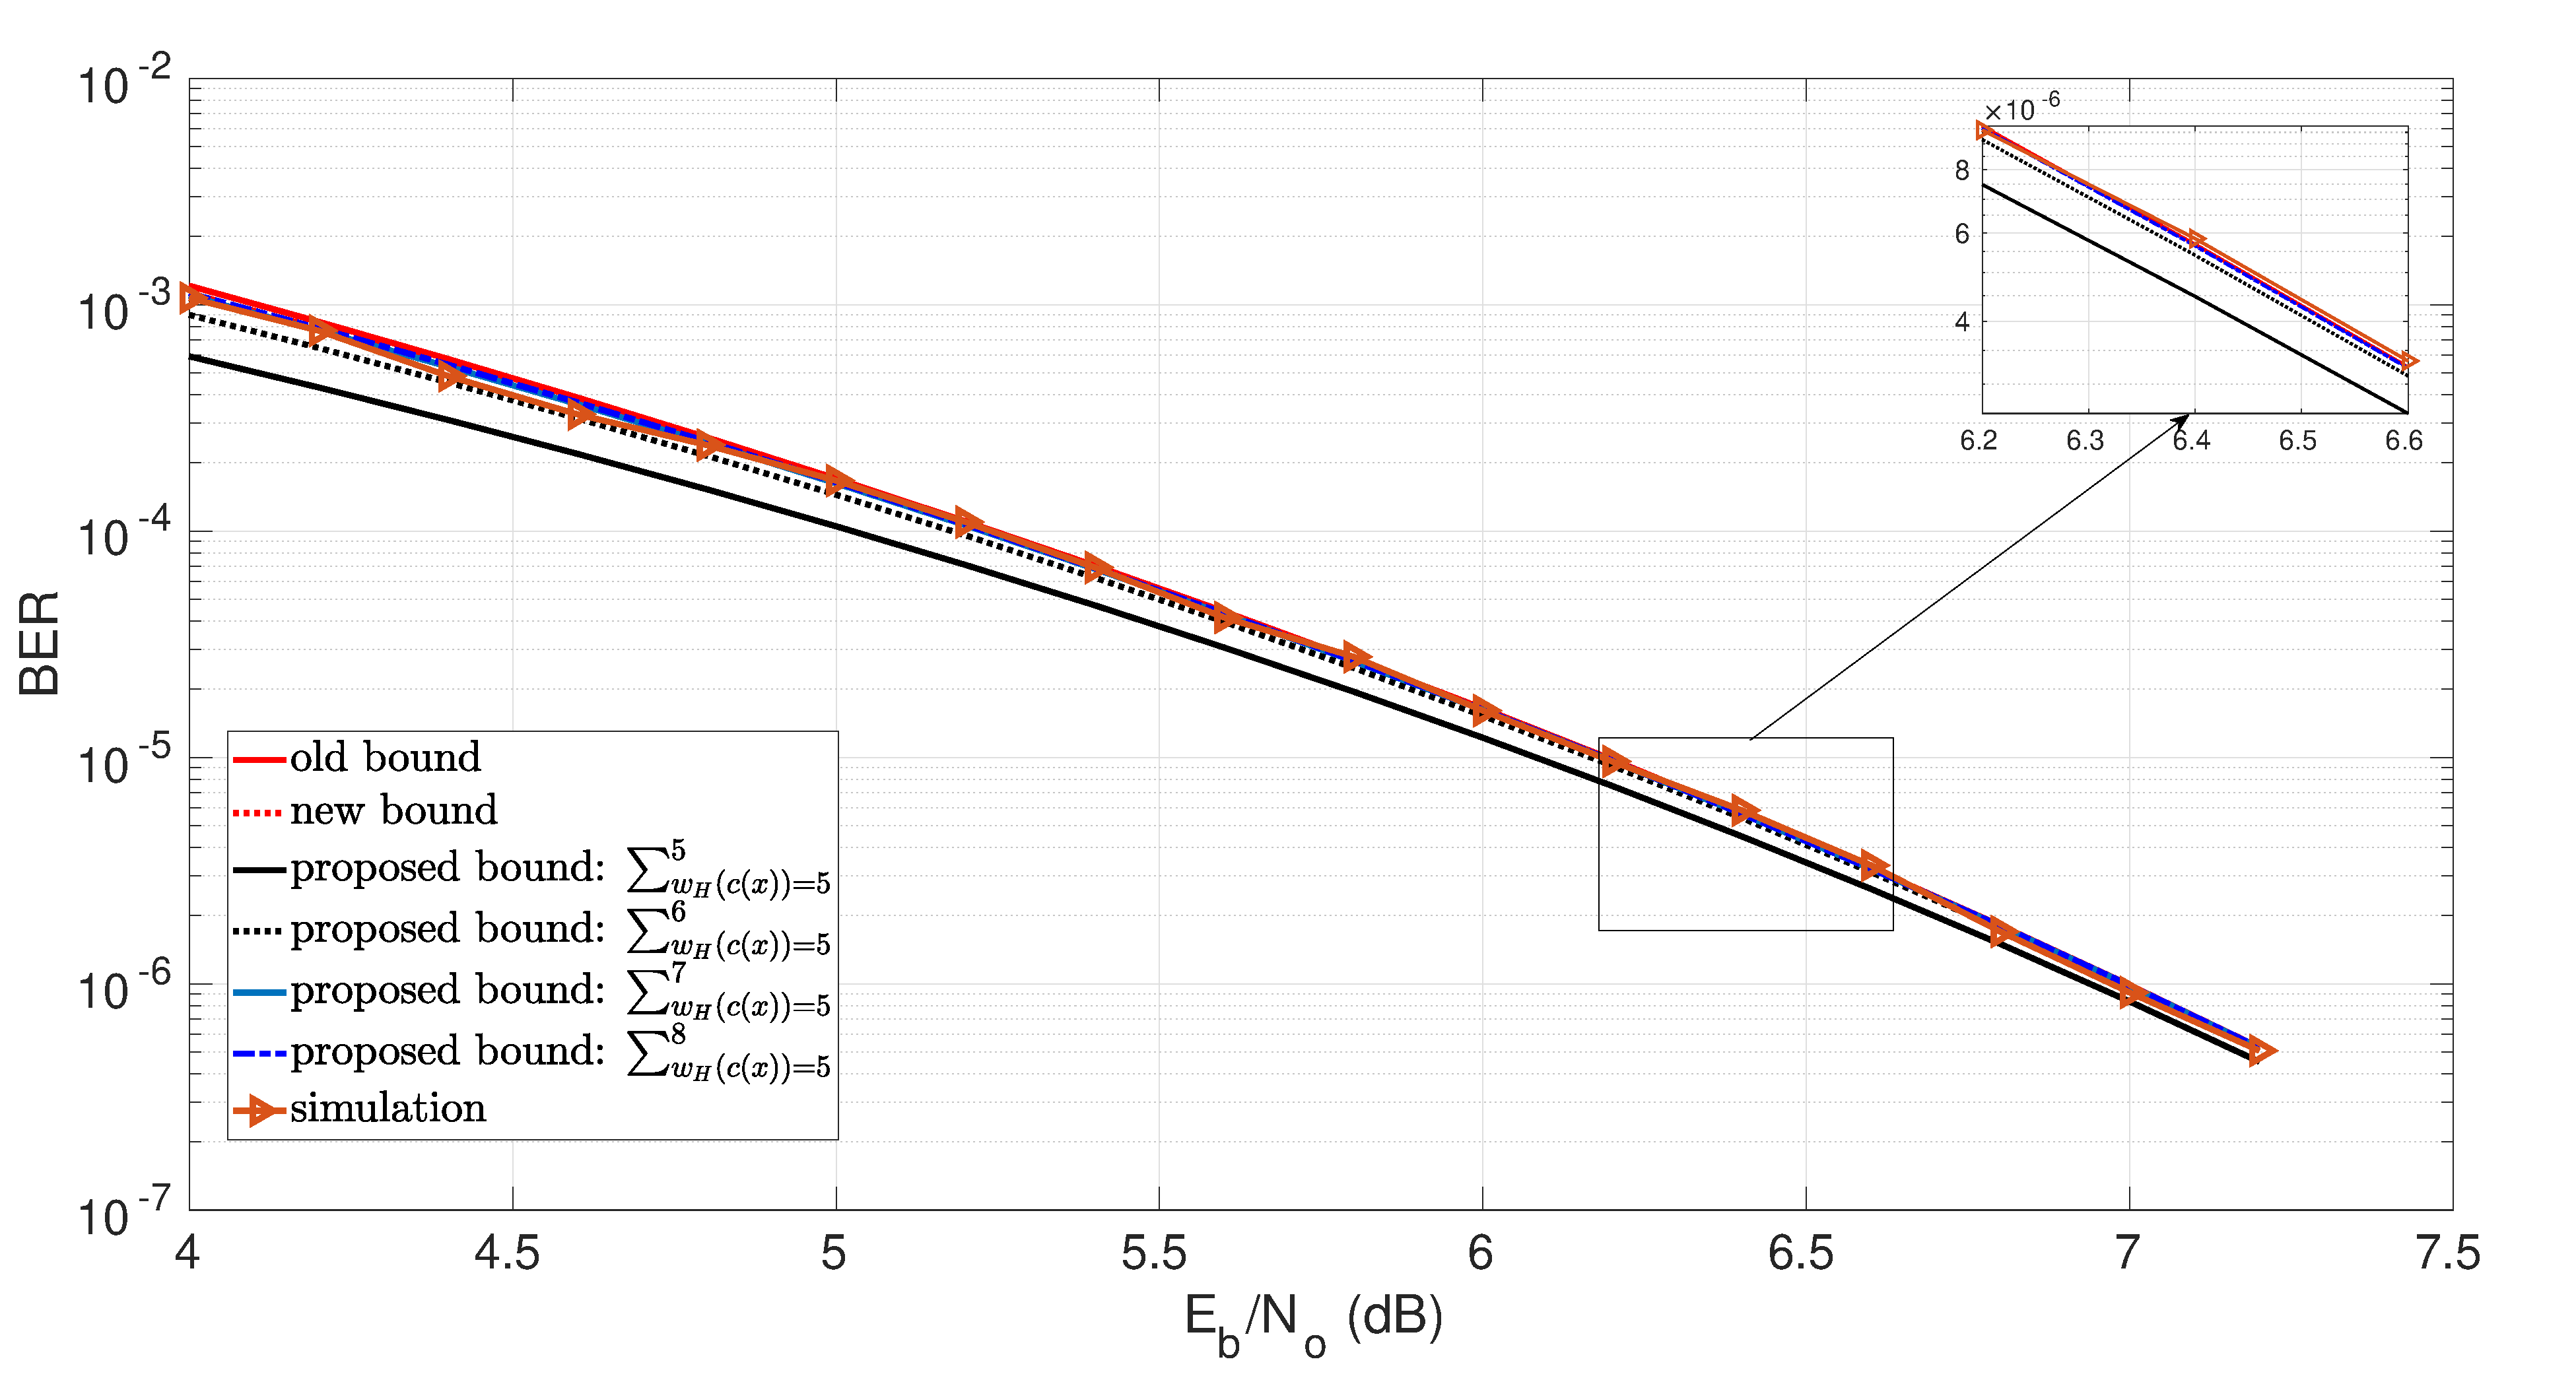
\includegraphics[width=0.5\textwidth]{./Images/RSC_5_7_lower_weights3.eps}
	\captionof{figure}{Old Bound vs New Bound vs Simulation for 5/7 RSC Code}
	\label{simFig1}
\end{figure}

As shown in Table \ref{code-tables-1}, since the free distance of the 5/7 RSC code is 5, and the codewords consisting of weigts 2 and 3 SCs or PCs are taken into account in the proposed method, all codewords with weights up to 7 are picked up. For the codewords of weight-8 on the other hand, some of them consisting of the weight-4 SC and PC are omitted in our method. However, Fig. \ref{simFig1} indicates that the union bound obtained using the codewords with weights up to $d_{\rm free+1}$ tracks the BER curve with sufficient accuracy, especially in the high $E_b/N_0$ region. Moreover, the bounds obtained by our method and the transfer function converge to the same value with $E_b/N_0$ increament and match the simulation results well. 

For the 37/21 RSC code, since the free distance of the code is 6, the counting omission in the proposed method occurs for the codewords with weight higher than 7. Although Table \ref{code-tables-2} indicates that there are 3 weight-8 codewords, and only one of them is found by our method, we can see from Fig. \ref{simFig2} that their contributions to the union bound are negligible and the BER curve can be well approximated using the codewords with weight 6 and 7 with a high accuracy at the high $E_b/N_0$ region.

\begin{figure}[htbp]
	\centering
	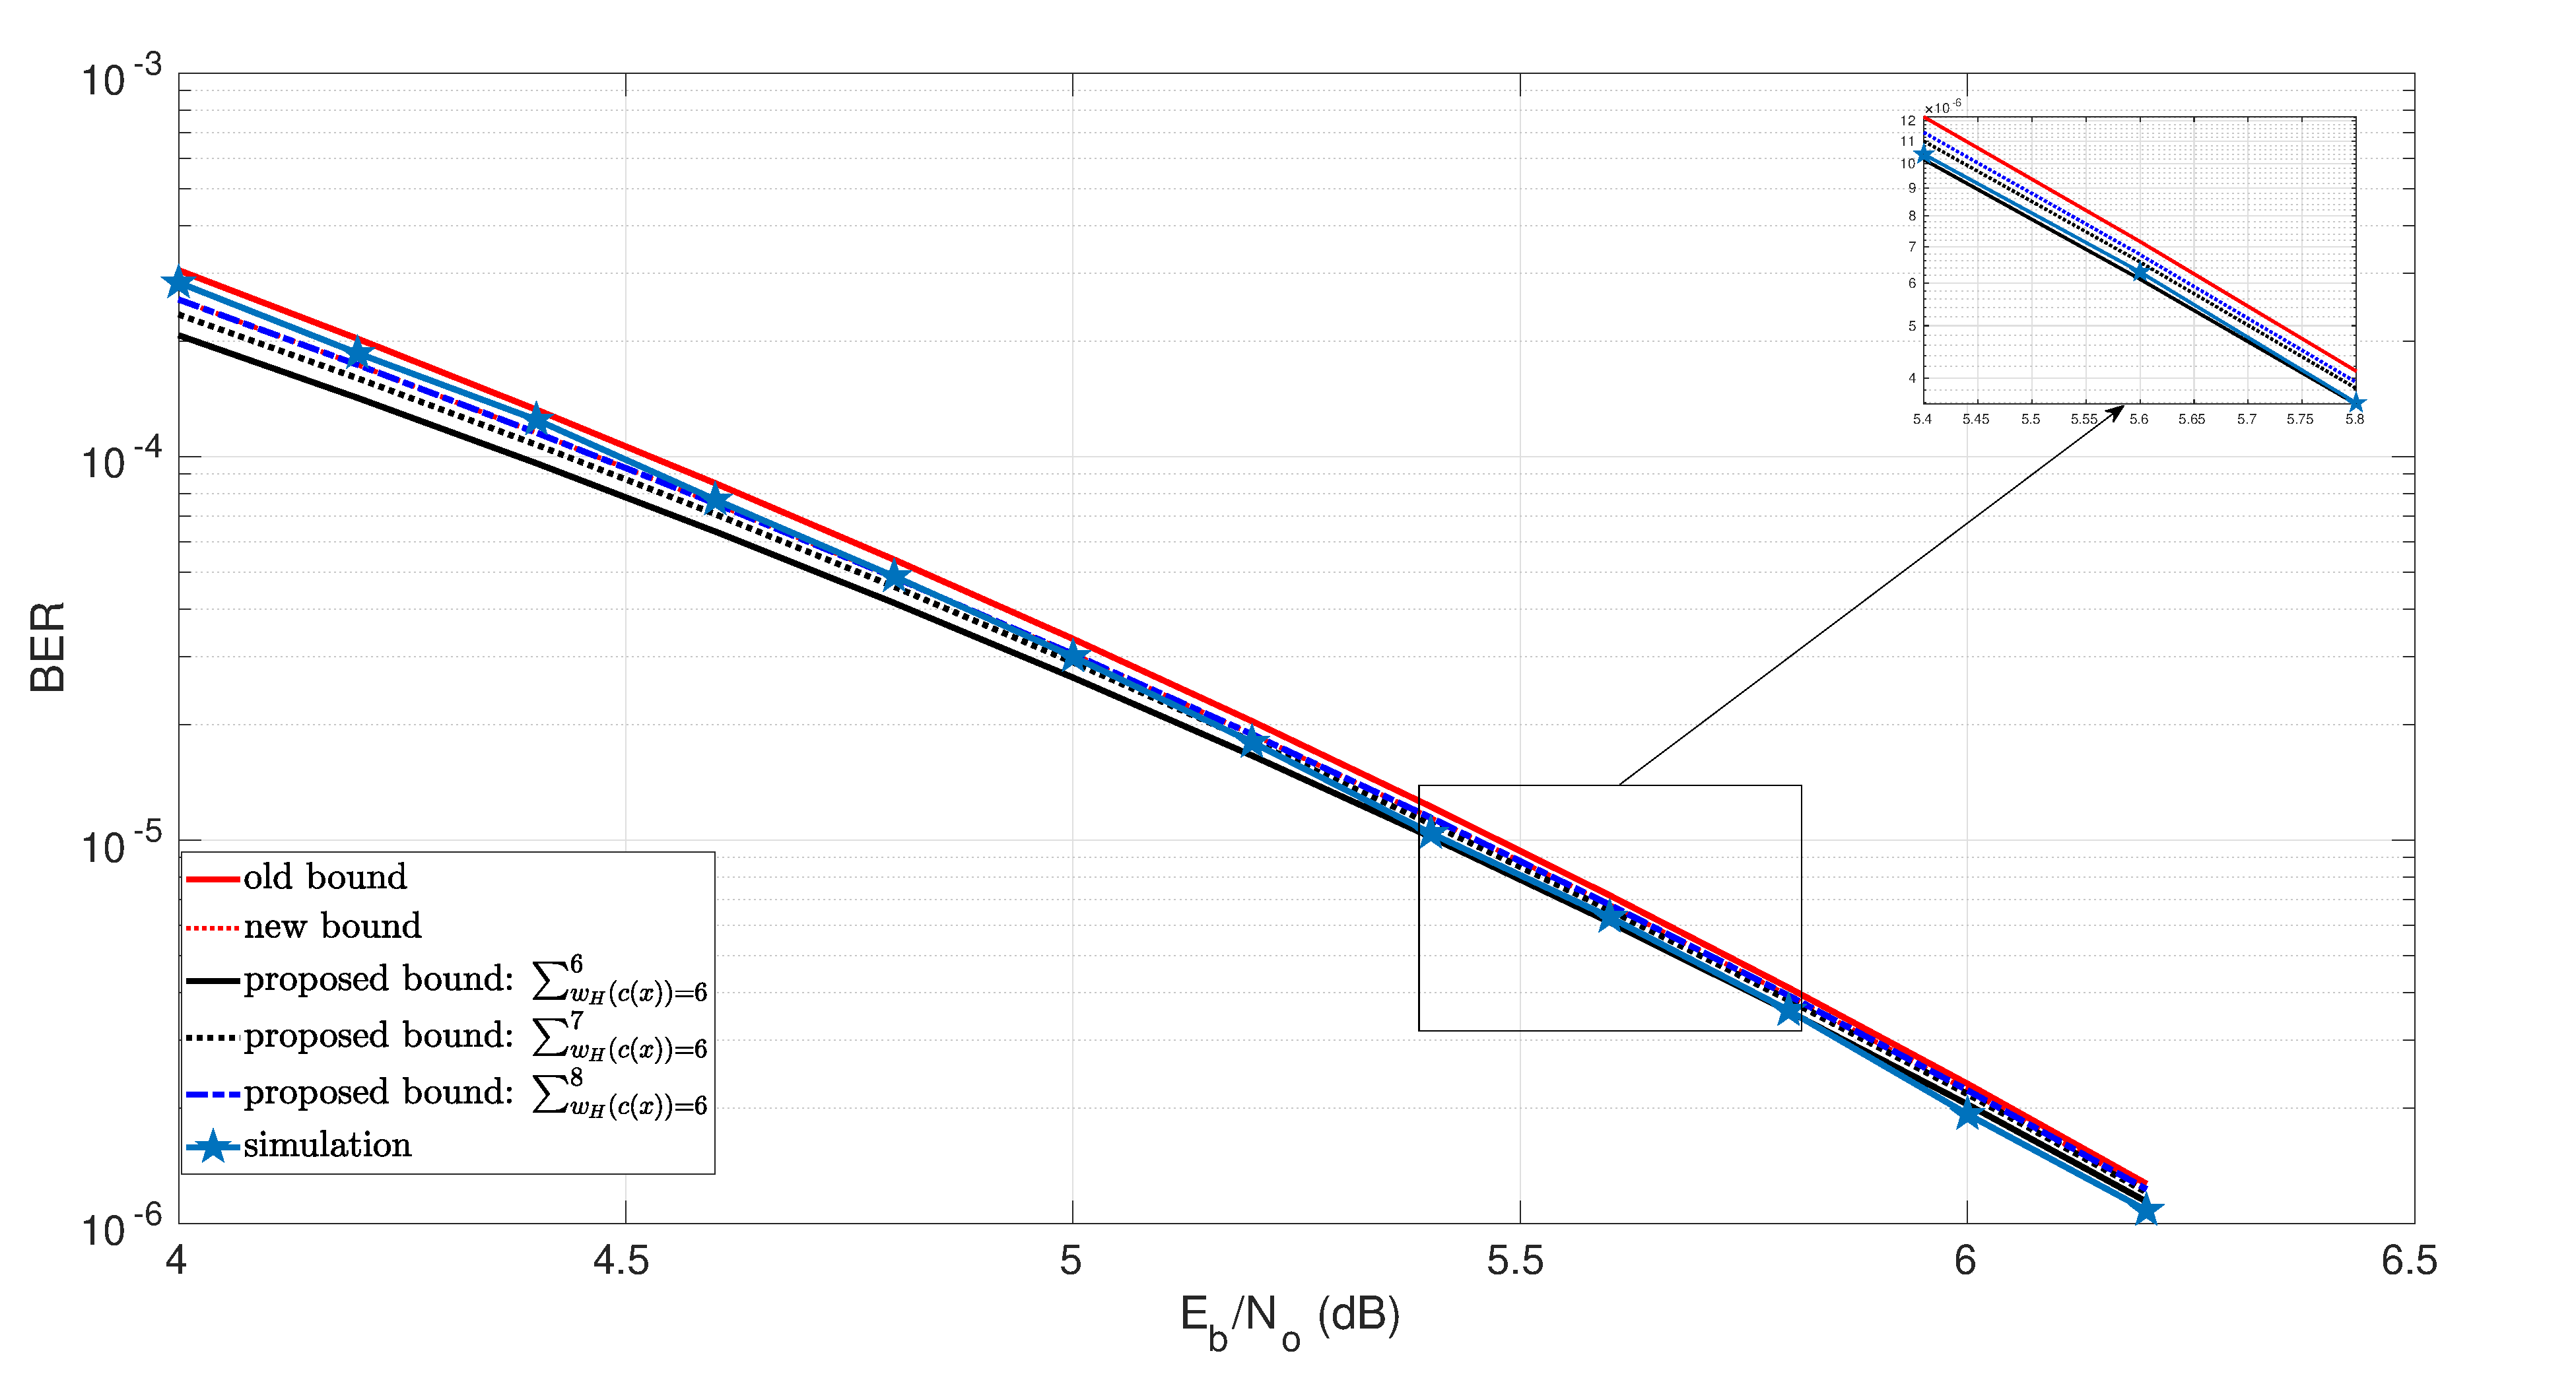
\includegraphics[width=0.5\textwidth]{./Images/RSC_37_21_lower_weights3.eps}
	\caption{Old Bound vs New Bound vs Simulation for 37/21 RSC Code}
	\label{simFig2}
\end{figure}

For the code III, the free distance is 7 and the proposed method identifies 2 codewords with weight-7 while 3 codewords with weight-8 can not be found as shown in Table \ref{code-tables-3}. Thus, while we use the weight-7 codewords to approximate the BER curve as Fig. \ref{simFig3}, there about a 0.1 dB gap between the proposed method and simulation results.

\begin{figure}[htbp]
	\centering
	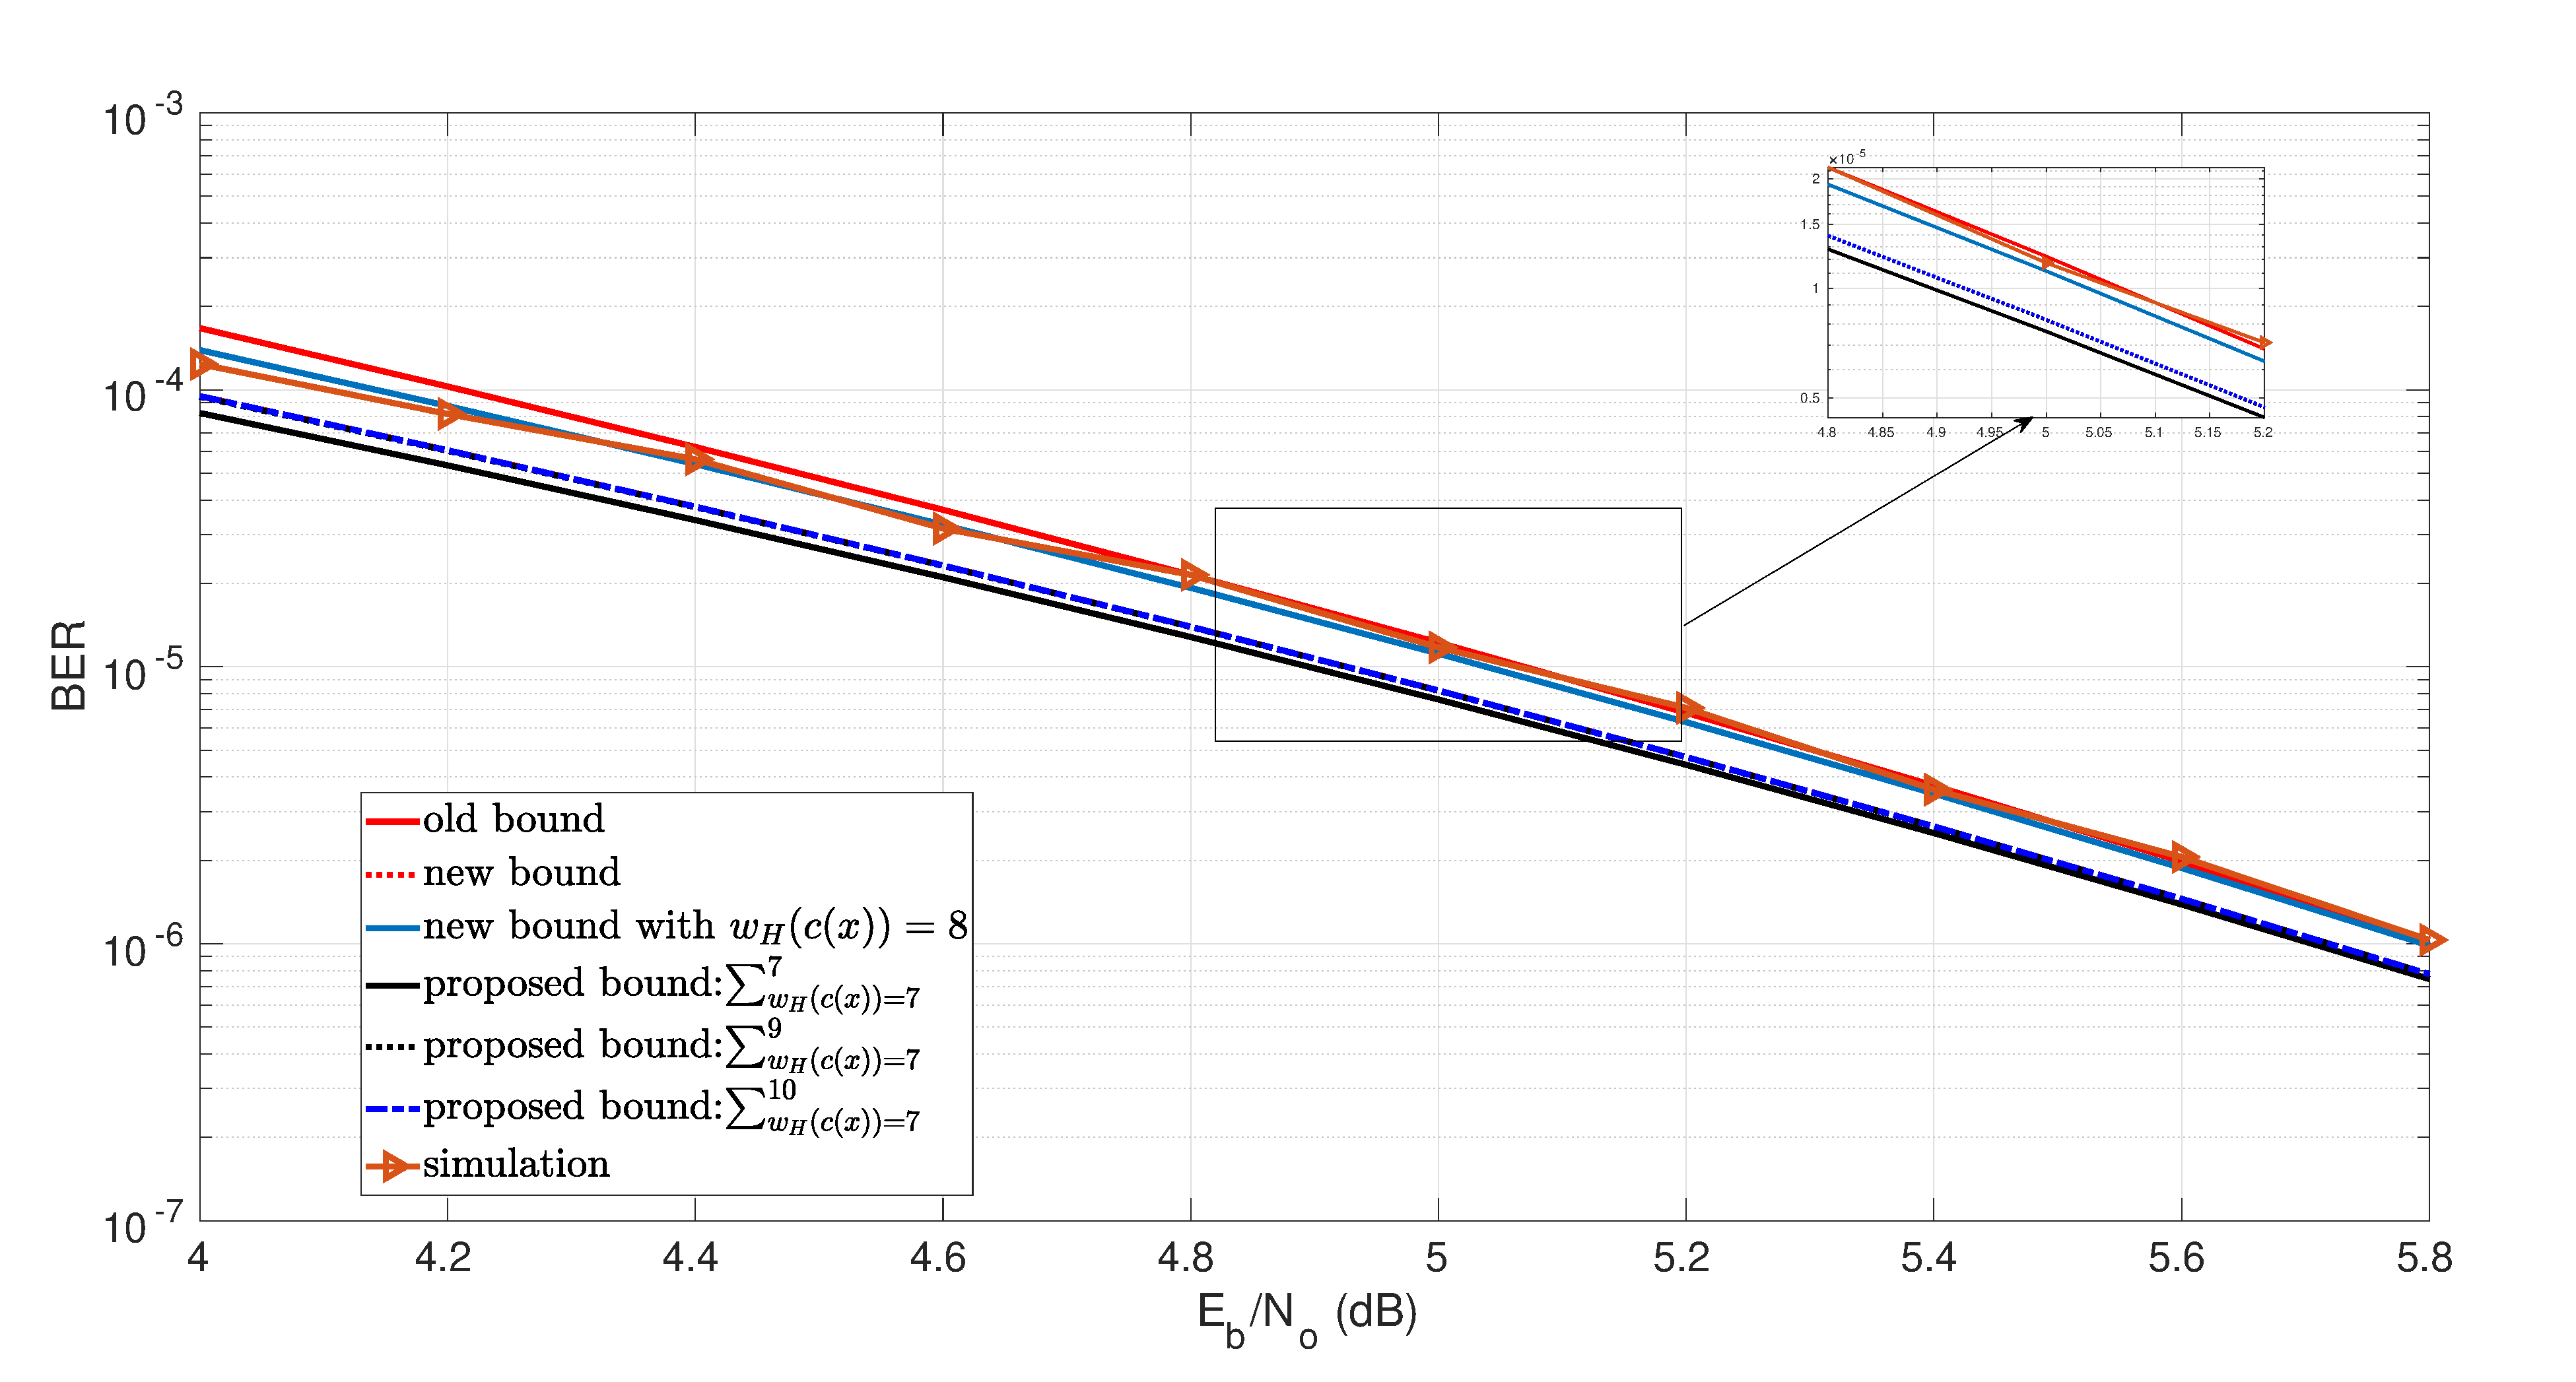
\includegraphics[width=0.5\textwidth]{./Images/RSC_23_35_lower_weights3.eps}
	\caption{Old Bound vs New Bound vs Simulation for 23/35 RSC Code}
	\label{simFig3}
\end{figure}






\section{Conclusion}
\label{sec6}
In this paper, we proposed a novel method for  listing the patterns of the SCs and PCs ($w_H(b(x)),w_H(h(x)) = 2,3$) of a low-weight RSC codeword, given the RSC code and a codeword cut-off weight, $d_{\rm free+1}$.
Compared to the transfer function method, it has low complexity and the knowledge of the SC and PC patterns makes it a very useful for interleaver design. To validate our method, we compared the union bound obtained using our novel method with the union bound obtained via the transfer function as well as the simulation results for three RSC codes. Results suggest that most RSC codes can be sufficiently characterized by our novel method.

\bibliography{\folder/reference/IEEEabrv,\folder/reference/References}
\end{document}